\documentclass[conference]{IEEEtran}
\IEEEoverridecommandlockouts
% The preceding line is only needed to identify funding in the first footnote. If that is unneeded, please comment it out.
\usepackage{cite}
\usepackage{amsmath,amssymb,amsfonts}
\usepackage{cite}
\usepackage{algpseudocode}
\usepackage{graphicx}
\usepackage{textcomp}
\usepackage{xcolor}
\usepackage{amsthm}
\usepackage{algorithm}
%\usepackage{algorithmic}
\usepackage{epstopdf}
\usepackage{subfigure}
\usepackage{verbatim}
\usepackage{diagbox}



\newcommand{\tabincell}[2]{\begin{tabular}{@{}#1@{}}#2\end{tabular}}
%\renewcommand{\bibfont}{\footnotesize}
\def\BibTeX{{\rm B\kern-.05em{\sc i\kern-.025em b}\kern-.08em
    T\kern-.1667em\lower.7ex\hbox{E}\kern-.125emX}}
\begin{document}

\title{Workload-Aware Scheduling for Data Analytics upon Heterogeneous Storage}

\author{\IEEEauthorblockN{Mingtao~Ji, Yibo~Jin, Zhuzhong~Qian, Sanglu~Lu}
\IEEEauthorblockA{State Key Lab. for Novel Software Technology, Nanjing University, Nanjing, China}
\{jmt, yibo.jin\}@smail.nju.edu.cn, \{qzz, sanglu\}@nju.edu.cn}


\maketitle
%Since the read speeds of diverse storage devices are quite different, the unbalanced use on either specific type of storage or particular device would easily overload them, making them being hotspots and finally worsen the read performance for analytical tasks.
\begin{abstract}
A trend in nowadays data centers is that equipped with SSD, HDD, etc., heterogeneous storage devices are widely deployed to meet diverse demands of various big data workloads. 
Since the reading performance of these storage devices are quite different, traditional concurrent data fetching easily incurs unbalanced use among devices, leading to the straggler in terms of the task reading time as well as elongating the overall latency for data analytics.
To avoid such unbalanced use on fetching large volume of data concurrently from storage devices, we formulate Workload-Aware Scheduling problem for Heterogeneous storage devices (WASH), which essentially minimizes the maximal task reading time for parallel data analytical tasks. Afterwards, we design a randomized algorithm ($r$WASH), which chooses source device for each task based on delicate calculated probabilities and can be proved concentrated on its optimum with high probability through our theoretical analysis. Extensive experiments show that $r$WASH reduces the average reading time for tasks by up to 55\% over the state-of-the-art algorithms.
%as well as show its NP-hardness

\end{abstract}

\begin{IEEEkeywords}
big data analytics, heterogeneous storage devices, workload-aware scheduling
\end{IEEEkeywords}

\section{Introduction}

Nowadays, there is a new trend that data centers have a variety of data analytical workloads, e.g., some data streaming applications like Storm
\cite{b40}, and other machine learning based applications like Grep \cite{b27}. Different workloads might have different requirements on storage performance \cite{b28} \cite{b29} \cite{b30} \cite{b31}. For example, Storm is a compute-intensive application whose computation significantly relies on the I/O performance while Grep is an I/O-intensive application which has high throughput on data processing. In order to meet these demands, a lot of heterogeneous storage devices \cite{b6} have been widely deployed for big data analytics frameworks within the cluster, e.g., Hadoop \cite{b14} and Spark\cite{b15}.

However, the heterogeneity of these devices easily leads to the divergent reading performance due to two main aspects. First, the different types of storage, e.g., SSD \cite{b32} and HDD \cite{b33}, naturally results in different reading performance. As shown in Fig.~\ref{Fig:motivation}, fetching the same amount of data from HDD takes almost twice longer than that from SSD. Second, the number of data fetching concurrently on a device also affects the I/O performance. As further shown in Fig.~\ref{Fig:motivation}, when the number of data fetching increases, the reading time also increases as a result of concurrent use.%when the number of tasks increases, the reading time for each task will also increase.
%when there are a large number of tasks reading data concurrently from specific device, read performance is also affected

% unbalanced usage on storage device
Essentially, different reading performance results from the unbalanced use on storage devices, but traditional strategies \cite{b2} \cite{b3} \cite{b4} \cite{b5} often ignore to avoid it  and incur relatively longer task reading time. More specifically, fetching data from the devices with higher I/O performance actually earns shorter task reading time than that from those with lower I/O performance \cite{b7}. However, crowded I/O requests on a particular device unfortunately elongate the task reading time and correspond data analytics, which should be avoid as much as possible. 

\begin{figure}[!t]
	\centering
	\includegraphics[height=1.8in]{fig_motivation5.eps}
	\caption{Comparisons of (1) reading time for one piece of data with unified size (64MB) on various storage, i.e., SSD and HDD. (2) reading time for various I/O workloads, i.e., the number of data fetching concurrently.}
	\label{Fig:motivation}

	%\vspace{-0.4cm}
\end{figure} 

%However, due to the divergent read performance of different storage and the cumulative workload of the storage, its hard to hard to achieve this aim. 
 
Thus, we propose to focus on dealing with unbalanced use on heterogeneous storage devices in this paper. However, due to the multiple replicas of data, how to choose target source from feasible devices storing the replica is also a big challenge.
Most of the previous researches have already focused on heterogeneous computing resources \cite{b25}\cite{b26}\cite{b35}\cite{b36}, but ignore the heterogeneous storage devices. Although some works have already considered heterogeneous storage devices \cite{b6}\cite{b7}, unbalanced I/O workloads and multiple data replicas are both not considered. In contrast, we formulate the Workload-Aware Scheduling problem for Heterogeneous storage devices. Afterwards, we propose a randomized algorithm ($r$WASH) with guaranteed performance by carefully choosing source device based on delicate calculated probabilities.
%as well as show its NP-hardness
%We focus on two aspects. One is the read performance of the disk itself, the other is the load of the disk, that is, the number of tasks that are reading the data from the disk. Focus on the above two points, we formulate it as an optimization problem and propose a heuristic algorithm (WASH-greedy) and a random algorithm ($r$WASH) with guaranteed performance to solve the problem. %Experiments show that the performance of the proposed algorithm is 55\% better than the Storage-unaware scheduling mechanism. 
More concretely, our contributions are as listed follows: 

\begin{itemize}
%\item We present the necessity of sloving this problem by showing impact of reading data phase during the task execution.
\item To balance the I/O workloads on heterogeneous storage devices, we propose Workload-Aware Scheduling problem for Heterogeneous storage devices (WASH).
%which is shown as a NP-hard problem 
\item We propose randomized algorithm with guaranteed-performance ($r$WASH), which can be proved concentrated around its optimum with high probability, i.e., 1 - O($e^{-t^2}$), where $t$ is the concentration bound.
\item The results of our extensive simulations show that our $r$WASH improves by up to 55\% over the art-of-the-state algorithm in terms of average tasks reading time.
%compared with the storage-unaware scheduling mechanism and by 20\% 
\end{itemize}

The rest of the paper is organized as follows. In Section \ref{RELATED_WORKS}, we present the related works of the WASH problem. 
Then the system model and algorithm are proposed in Section \ref{SYSTEM_MODEL} and Section \ref{DESIGN_ALGORITHM}, respectively. 
In Section \ref{Analysis}, the theoretical analysis of proposed $r$WASH is presented.
At last, we conclude this paper in Section \ref{CONCLUSION} by summarizing our main contributions.


\section{RELATED WORKS}\label{RELATED_WORKS}
The related works are summarized from two main parts. For the first part, due to limited bandwidth, some works focus on data locality \cite{b2} \cite{b3} \cite{b4} \cite{b5} to reduce data transmission of data analytics. However, in heterogeneous scenario, it is not enough to consider data locality alone. Thus, some other studies \cite{b1} \cite{b6} \cite{b19} \cite{b8} have been carried out to accelerate data analytical tasks by considering hardware heterogeneity.

\textbf{Fetching Data Locally.} Due to limited network bandwidth in data center, a large amount of data transmitted between nodes before task execution, greatly affects the performance of data analytics. Therefore, processing data locally as much as possible actually improves the performance, e.g., deploying tasks to the nodes where the input data is stored. 
%delay when the job that should be scheduled next according to fairness cannot launch a local task, it waits for a small amount of time, letting other jobs launch tasks instead
In order to improve data locality, Matei \cite{b2} proposed delay scheduling, which keeps jobs waiting for a while until queuing delay reaches to a presetted threshold or there is idle resource at local.
%a little time instead of launching local tasks when local resources are scarce. %can't launch a local task. Delay scheduling considers that when a node has idle slots, priority should be given to  the tasks whose input data is stored at that node, and delay to schedule tasks whose related data is not stored at that nodes. 
Ganesh \cite{b3} made multiple replicas for frequently used data by analyzing the number of their accesses, improving the data locality. 
Cristina \cite{b4} proposed a distributed adaptive data replication algorithm DARE, which helped the scheduler for better data locality. 
Jalaparti \cite{b5} believed that most of the production workloads are repetitive and predictable, by which the scheduler could make scheduling plan ahead. 
%Coordinating the tasks and data placement of these jobs can effectively reduce bandwidth usage, further, improving data locality. 
All of these works improves the performance of data analytics by considering data locality. 
However, due to the fact that local disks might have high I/O workloads, previous strategies would elongate the reading time of local tasks.

\textbf{Fetching Data Remotely.} 
In heterogeneous cluster, data fetching remotely from those devices with higher performance on I/O could be better than that from local ones.
%since tasks fetching data from high-performance disks of other nodes might have low reading time, considering data locality alone is not enough to speed up analytical tasks. 
However, most of the researches only focused on heterogeneous computing resources \cite{b25} \cite{b26} \cite{b35} \cite{b36} \cite{b6}, but ignored the heterogeneous storage devices. For example, Xu \cite{b6} considered the current usability of underlying hardware (CPU, memory, I/O), but didn't consider the performance on different storage hardware. 
In Hadoop 2.3, HDFS\cite{b19} took the heterogeneous storage feature into consideration, which supported six storage strategies. Users could choose one of these strategies to store files according to their demands.
%is proposed considers heterogeneous storage devices and supports multiple storage strategies. One of the storage strategies is named , that is, one replicas is stored in SSD, and the rest is stored in HDD. 
%However, the task scheduling strategy is not aware of the disk's performance.
Based on such feature, Pan \cite{b7} proposed H-Scheduler to launch tasks according to the different performance between HDD and SSD. However, such scheduling mechanism used heuristic method to read data from HDD or SSD, ignoring unbalanced use among disks.
%However, with the increasing trend of heterogeneous storage devices, it is one-sided to divide the storage devices into two categories. 
Wang B \cite{b8} used Markov to model the use of nodes in the cluster to deploy data reasonably, but ignored the tasks reading time and the heterogeneity of devices. %However, the scheduling problem of reading tasks is not considered, and the heterogeneity of different storage media is not considered, either. %These works do not accurately define the differences between storage hardwares, and there is still a situation where a large number of tasks read data from low-speed devices, causing bottlenecks.
%in a blind way

Among these works, either the reading time of the tasks or the target disks is not considered. Thus, there is still a situation where a large number of tasks overload storage devices, causing bottlenecks.
The difference between those works and ours is that our work specifically models the reading differences and the I/O workloads among disks. Then, each task chooses source disks based on delicate calculated probabilities, to speed up its reading time.

\section{SYSTEM MODEL AND PROBLEM FORMULATION}\label{SYSTEM_MODEL}
In this section, we first introduce the background of heterogeneous storage devices used in data analytics and then build the system model. After that, we formulate the Workload-Aware Scheduling problem for heterogeneous devices.
%and show its NP-hardness 

\subsection{Background and motivation}\label{AA}

In data center, Hadoop and Spark widely use heterogeneous storage devices to support different workloads. For example, in MapReduce framework, Shuffle stage \cite{b42} \cite{b41} usually has a large requirement on I/O for storing intermediate data. In order to meet this demand, Crail \cite{b37} is proposed to be a high-performance I/O architecture for data processing, using NVMe SSD \cite{b45} as a supplementary to speed up Shuffle phase.
%with the number of heterogeneous disks increasing, traditional scheduling may lead to disk bottleneck. Before analysing the problem, we will introduce data and replicas as well as job and tasks first.

\textbf{Data and replicas.} In data analytics system, large volume of data is generated, such as GPS information\cite{b38}, system logs\cite{b39}, etc. Due to their massive sizes, a large file is often divided into multiple fixed-size pieces, i.e., one $data$ block, stored in a distributed file system such as HDFS \cite{b19}, whose uniform size is often 64MB or 128MB. However, the disk is usually unreliability, e.g., about 5 to 6 disks are damaged per day in a cluster of 5,000 machines \cite{b32}. In order to avoid such data loss, traditional approach is to keep multiple $replicas$ of each data in storage, e.g., three backups across two racks \cite{b19}. Then, one piece of data will be stored in multiple disks with various I/O performance.
% The tasks will be scheduled to node to execute. ,

\textbf{Job and tasks.} A data analytics workload, named a $job$, includes many parallel $tasks$. Since each task must read its related input data before execution from the corresponding disk, the scheduler in data analytics system needs to decide the source device for each task among multiple replicas. Note that the completion of a job relies on the most straggling task.
%Note that the completion of a job is determined by stragglers: tasks that take much longer to complete than other tasks in the job.


However, traditional schedulers for data analytics are usually unaware of disks' types and I/O workloads, which often leads to straggler tasks. In contrast, our scheduler is then designed to avoid the stragglers by balancing I/O workloads among heterogeneous storage devices.

\textbf{Motivation and example.}
%In order to improve the performance of data analytics tasks, tasks should read data from high performance and low load disks. 
We will use a simple example to illustrate the importance on choosing heterogeneous storage devices. As shown in Fig.~\ref{Fig:example}, there are two types of disks, i.e., SSD and HDD. The reading time for a data replica from SSD and HDD is $T_1 = 0.2s$ and $T_2 = 0.4s$, respectively. 
\begin{itemize}
	\item The traditional scheduler deploys tasks like scheduling \uppercase\expandafter{\romannumeral1} of Fig.~\ref{Fig:example}(a), whose reading time for a data replica is $0.4s$ while the reading time of the delicate method, i.e., scheduling \uppercase\expandafter{\romannumeral2}, is $0.2s$. Obviously, the task that reads data from SSD has a shorter reading time than that from HDD, i.e., scheduling \uppercase\expandafter{\romannumeral2} is better than scheduling \uppercase\expandafter{\romannumeral1}.

	\item In Fig.~\ref{Fig:example}(b), since the number of fetching data concurrently is 3 from SSD, the reading time of scheduling \uppercase\expandafter{\romannumeral1} is then $0.2s * 3 = 0.6s$, while the task reading time of the delicate method, i.e., scheduling \uppercase\expandafter{\romannumeral2}, is $max\{0.2s * 2, 0.4s\} = 0.4s$. Apparently, the tasks that read data from such storage device with a lower I/O workloads have a shorter reading time than that from higher ones, i.e., scheduling \uppercase\expandafter{\romannumeral2} is better than scheduling \uppercase\expandafter{\romannumeral1}.
\end{itemize}

This simple case reveals two important findings: (1) The types of heterogeneous storage devices affect task reading time. (2) The I/O workloads of storage devices also have effects on task reading time. In order to shorten the task reading time, we should take both of the these two findings into consideration.

%\begin{figure}[!t]
%\begin{minipage}[!t]{0.51\textwidth}
%	\centering
%	\subfigure[Type of storage. Scheduling 1 = $0.4s$, Scheduling 2 = $0.2s$]{\label{Fig:example1}\includegraphics[height=1.1in]{fig_example1_3.eps}}	
%	\subfigure[Load of storage.  Scheduling 1 = $0.2s*3$, Scheduling 2 = $max\{0.2s*2, 0.4s*1\}$]{\label{Fig:example2}
%	\includegraphics[height=1.1in]{fig_example2_2.eps}}
%	\caption{Two aspects that affect the task reading time: (1) type of storage, \protect\\(2) Load of storage. Delicate method, i.e., Scheduling 2, improves 50\%, 33\% over scheduling 1, respectively.}
%	\label{Fig:example}
%\end{minipage}
%\end{figure}
%width=4.78cm width=3.95cm

\begin{figure}[!t]
\centering
    \begin{minipage}{4.78cm}
        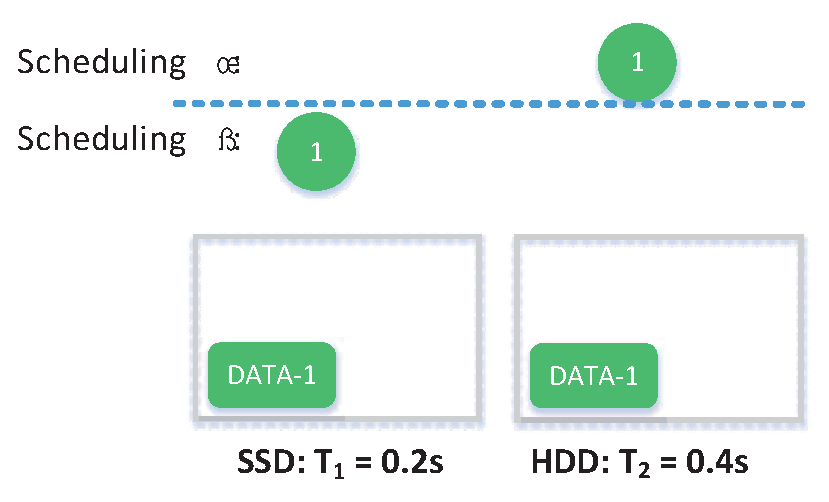
\includegraphics[height = 2.8cm]{fig_example1_5.eps}
        \centerline{\footnotesize{\uppercase\expandafter{\romannumeral1} : $max$\{$0s$, $0.4s$\},\quad}}\\
        \centerline{\footnotesize{\uppercase\expandafter{\romannumeral2} : $max$\{$0.2s$, $0s$\}.\quad}}\\
         \centerline{(a) Type of storage.}\\
    \end{minipage}
    \begin{minipage}{3.95cm}
        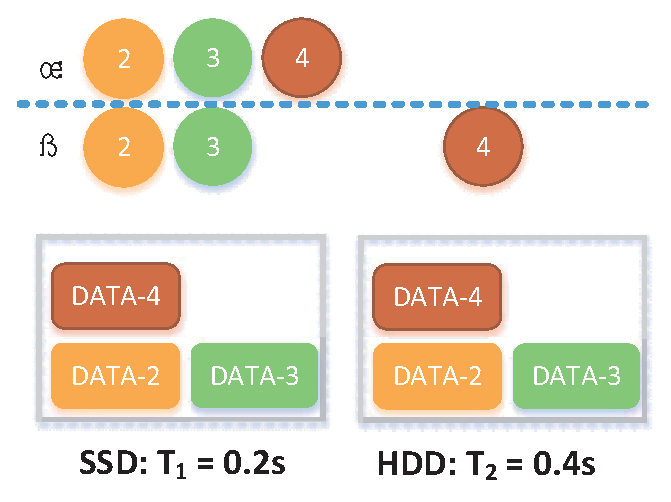
\includegraphics[height = 2.8cm]{fig_example2_4.eps}
        \centerline{\footnotesize{\uppercase\expandafter{\romannumeral1} : $max$\{$0.2s*3$, $0s$\},\quad}}\\
        \centerline{\footnotesize{\uppercase\expandafter{\romannumeral2} : $max$\{$0.2s*2$, $0.4s$\}.}}\\
         \centerline{(b) Load of storage.\quad}\\
    \end{minipage}
    \vspace{-0.4cm}
    \caption{Two aspects that affect the task reading time: (a) Type of storage, (b) Load of storage. Delicate method, i.e., Scheduling \uppercase\expandafter{\romannumeral2}, improves 50\% and 33\% over scheduling \uppercase\expandafter{\romannumeral1}, respectively.}
    \label{Fig:example}
    \vspace{-0.4cm}
\end{figure}

%denoted by \{$r_l^1$, $r_l^2$,... $r_l^{C}$\}
\subsection{System Model}

The major notations used are listed in Table~\ref{table-notations}. The data center is equipped with heterogeneous disks, hence we denote by $\mathcal{D}$ the heterogeneous disks set, i.e., $\mathcal{D}$ = \{1, 2, ...,$|\mathcal{D}|$\}. Each disk-$i$ corresponds to a different reading time for only one replica as its reading performance, represented by $T_i$, $i \in \mathcal{D}$.
$\mathcal{M}$ is defined as the set of all data in data center, $\mathcal{M}$ = \{1, 2, ..., $|\mathcal{M}|$\}. Each data-$l$ has $C$ replicas stored in $C$ different disks whose size is $\tau$, e.g., 64MB. $\pi_l^{i}$ is a binary variable indicating whether data-$l$ is stored in disk-$i$ or not. More concretely, we define $\pi_l^{i}$ as
\begin{equation}
\pi_l^{i} =
\begin{cases}
1, &\text{if disk-$i$ stores a replica of data-$l$,}\\
0, &\text{otherwise.}
\end{cases}\nonumber
\vspace{-0.2cm}
\end{equation}

For each of submitted job, it is often divided into parallel tasks by data analytics framework, denoted by $\mathcal{T}$ = \{1, 2,  ..., $\mathcal{|T|}$ \}. Each task-$j$ corresponds to an input data whose index is defined as $\phi_j$. Since there are $C$ replicas for each data stored in different $C$ disks, task-$j$ can read data-$\phi_j$ among those $C$ disks, whose indexes can be represented as \{$d_{1}^j$, $d_{2}^j$,... $d_{C}^j$\}.


$I_i^j$ is a decision variable, indicating whether task-$j$ chooses the replica stored in disk-$i$ as its input or not. Specifically, we define $\pi_l^{i}$ as
\begin{equation}
I_i^j =
\begin{cases}
1, &\text{\tabincell{l}{if task-$j$ chooses the replica stored in disk-$i$,}}\\
0, &\text{otherwise.}
\end{cases}\nonumber
\end{equation}

Then, we denote by $load_i$ the reading time of all tasks from disk-$i$, i.e.,
\begin{equation}
 load_{i} = \sum_{j}I_i^j*T_i. \nonumber
\end{equation}
 
 \vspace{-0.2cm}
 In order to balance the use on heterogeneous storage devices as well as optimize the reading time of data analytical tasks, our objective is to minimize the maximal $load$ of all disks.

\begin{table}[!t]
	\Large
	\centering
	\footnotesize
	\renewcommand\arraystretch{1.2}
	\caption{MAJOR NOTATIONS USED IN THIS PAPER.}
	\label{table-notations}
	\begin{tabular}{c|l}
		\hline\hline
		Variable & Description\\
		\hline
		$T_{i}$ & \tabincell{l}{The time of reading one replica from disk-$i$ \\for only one task without other concurrent tasks} \\
		\hline
		$\phi_j$ & The index of data that task-$j$ needs, as its input \\
		\hline
		$d_{r}^j$ & \tabincell{l}{The index of disk which stores data-$\phi_j$'s $r$-th replica} \\
		\hline
		$\pi_{l}^{i}$ & \tabincell{l}{A binary variable indicating if data-$l$ are \\stored in disk-$i$ or not} \\
		\hline
		$N_i$ & Number of tasks which reads data from disk-$i$ \\
		\hline
		$\tau$ & Unified size of each data replica in data center \\
		\hline
		$C$ & The number of replicas for each data \\
		\hline\hline
		Decision  & Description\\
		\hline
		${I}_i^j$ & \tabincell{l}{A decision variable indicating whether task-$j$ chooses \\the replica stored in disk-$i$ as its input or not}\\
		\hline	
	\end{tabular}
	\vspace{-0.4cm}
\end{table}

\subsection{Workload-Aware Scheduling problem for Heterogeneous storage devices $(\rm{WASH})$} \label{WASH}
%$\mathcal{AP} \mathbb{AP}$ (~/~)
%A large number of tasks are running in the cluster of data centers.
For parallel tasks, if the scheduler is unaware of the different reading performance of heterogeneous disks, it would easily lead to the unbalanced use on disks, elongating the reading time of analytical tasks. To avoid such bottleneck, we propose Workload-Aware Scheduling problem for Heterogeneous storage devices (WASH) whose goal is to minimize the maximal reading time. Detailed description is illustrated as follows:
%Finally, by determining the value of the decision variable $I_i^j$, the appropriate disk is selected for each task to read the corresponding data. Detailed description is as follows:
\begin{align}
Min:&\;\;\;\;\;\max\limits_{i}\{\sum_{j}I_i^j*T_i\}\;\;\;\;\;\;[\rm{WASH}]\nonumber\\
s.t. 
&\;\;\;\;\;\sum_{i}I_i^j = 1,\;\;\forall j,\label{task-cons}\\
&\;\;\;\;\;I_i^j \leq \pi_{\phi_j}^{i},\;\;\forall i,j\label{data-cons},\\
&\;\;\;\;\;I_i^j\in\{0,1\},\;\;\forall i,j.\label{def-cons}
\end{align}

%Constraint (\ref{task-cons}) guarantees that task-$j$ can only fetch data $\phi_j$ from those source disks. Constraint (\ref{data-cons}) guarantees that task-$j$ can only select from those disks containing its input data. If one replica of data $\phi_j$ is stored in disk-$i$, then $\pi_{\phi_j}^{i}$ = 1, otherwise $\pi_{\phi_j}^{i}$ = 0. Constraint 3 denotes the domain of decision variables, which can only be 0 or 1. $I_i^j$ = 1 indicates that task-$j$ selects the replica stored on disk-$i$ as input, while $I_i^j$ = 0 is on the contrary.The key to solve WASH problem is to determine the value of decision variables {$I_i^j$}. 
Constraint (\ref{task-cons}) and Constraint (\ref{data-cons}) guarantee that task-$j$ only fetches data-$\phi_j$ from one of those source disks storing its input. 
%$\phi_j$ represents the index of data that task-$j$ needs, $\phi_j$ $\in$  $\mathcal{M}$.
If one replica of data-$\phi_j$ is stored in disk-$i$, then $\pi_{\phi_j}^{i}$ = 1, otherwise $\pi_{\phi_j}^{i}$ = 0. 
The key to solve WASH problem is to determine the value of those decision variables, i.e., $I_i^j$. However, in general case, the optimization with integral decisions is NP-hard~\cite{b9}.

%Next, we show the NP-hardness of this problem. More specifically, WASH problem can be reduced from the integer linear programming (ILP) problem. The ILP problem is NP-hard \cite{b9} in general, so as that WASH problem is then NP-hard. The specific proof is as shown follows.

%\emph{\textbf{Theorem 1:}} The WASH problem is NP-hard.

%\emph{Proof:} See Appendix.

%Alogoritm1
\begin{algorithm}[!t]

	\textbf{Require:} Task-$j$ and its input data-$\phi_j$, $\forall j$.

	\begin{algorithmic}[1]
		
		\State $Result$ $\gets$ \{\}\label{WASH-greedy:init}
		\For{each task-$j$} 
			\State \{$d_{1}^j$, $d_{2}^j$,... $d_{C}^j$\} = $f(\phi_j)$
		
			\leftline{\;\;\;\;\;\;$//$ $f(\phi_j)$ is a set of disks storing data-$\phi_j$.}
	
			\State $d_{min}^j$ $\gets$ $\mathop{\arg\min}\limits_{d \in \{d_{1}^j, d_{2}^j,... d_{C}^j\}}$ $\{T_d\}$
			\State $Result$ $\gets$ $Result$ $\cup$
			\{$< j, d_{min}^j>$\}
		\EndFor
%\left \langle \right \rangle
	\State  Each task-$j$ reads data according to $Result$.
	\end{algorithmic}
	\caption{WASH-greedy}\label{WASH-greedy}
\end{algorithm}

\section{Design of Randomized Schema}\label{DESIGN_ALGORITHM}

The key to minimize the overall reading time for each task is to find the optimal source disk storing its input among heterogeneous disks. However, due to its inherent complexity of integral decisions for scheduling, the optimal solutions is hard to be obtained. Since it takes less time to read data from disks with higher I/O performance than that from those with lower I/O performance, we first explore a heuristic algorithm intuitively, which often chooses these disks with higher I/O performance, named WASH-greedy. However, due to its preference on high I/O performance disks, WASH-greedy may easily overload these disks, making them being bottlenecks. 
%However, due to the NP-hardness of WASH problem, the optimal solutions can't be obtained within polynomial time, unless NP $=$ P
%such algorithm always giving preference to disks with high-performance as input for each task
%However, extensive experiments shows that WASH-greedy has a little improvement over the baseline, i.e., Hadoop-default which is storage-unaware. 
Furthermore, to solve WASH effectively as well as to avoid bottlenecks, we design a randomized algorithm ($r$WASH) which chooses source devices based on delicate calculated probabilities and can be proved concentrated on its optimum with high probability, i.e., 1- O($e^{-t^2}$), through our theoretical analysis.

\subsection{Greedy-based Inspiration}\label{Heuristic}
%we first introduce WASH-greedy which is based on a greedy idea that always selects source disk with minimal reading time, i.e. $T_i$, greedily . 
In this subsection, we first introduce WASH-greedy which selects source disk with minimal reading time, i.e. $T_i$, greedily.

Algorithm \ref{WASH-greedy:init} shows the details of WASH-greedy. Line 1 initializes $Result$ = \{\}. Lines 2-6 are used to select a source disk for each task-$j$. In line 3, function $f$ is used to find the indexes of those disks which store the input data of task-$j$, i.e., data-$\phi_j$, represented by \{$d_{1}^j$, $d_{2}^j$,... $d_{C}^j$\}. Next, in line 4, the disk with minimal $T_i$ is selected from those $C$ disks. After $\mathcal{|T|}$ iterations, the selections of source disks for $\mathcal{|T|}$ tasks are completed. Then, each task will read its input data according to $Result$, as shown in line 7.

% After putting the task-$j$ and disk $d_{j_l}$ into the set $Result$, the algorithm completes one assignment of a task.

%Next, an example is given to illustrate the algorithm. In datacenter, there exits a set of heterogeneous disks $\mathcal{D}$= \{$d_1$, $d_2$, $d_3$, $d_4$\} with $T_i$ $T_1$ = 0.3,  $T_2$ = 0.1,  $T_3$ =0.2 and $T_4$ =0.2, respectively. Data set $\mathbb{M}$ = \{$m_1$, $m_2$, $m_3$, $m_4$\} are stored as Fig.\ref{fig1}. Obviously, each data has two replicas. When query tasks $\mathcal{T}$= \{$t_1$, $t_2$, $t_3$, $t_4$\} ($\phi_j$ = j, 1$\leq$j$ \leq$4) comes, the algorithm WASH-greedy runs as follows: %($\phi_j$ = j (1 $\leq$j$ \leq$ 4, task $t_j$'s input is $m_j$ which equals the DATA-j in Fig.\ref{fig1}))

Next, we use an example to illustrate the process of WAHS-greedy. In data center, there are four heterogeneous disks, i.e., $\mathcal{D}$= \{1, 2, 3, 4\}, with $T_1 = 0.2s$,  $T_2 = 0.25s$,  $T_3 = 0.4s$ and $T_4 = 0.6s$, respectively. Furthermore, five pieces of data are stored as shown in Fig.~\ref{fig1}. When a job with five tasks comes, algorithm WASH-greedy runs as follows: %Obviously, each data has two replicas. When query tasks $\mathcal{T}$= \{1, 2, 3, 4\} ($\phi_j$ = j, 1$\leq$j$ \leq$4) comes, the algorithm WASH-greedy runs as follows: %($\phi_j$ = j (1 $\leq$j$ \leq$ 4, task $t_j$'s input is $m_j$ which equals the DATA-j in Fig.~\ref{fig1}))

Initial: Result = \{\}
\begin{itemize}
	\item \textbf{Round 1}:for task-1:
	 f($\phi_1$) = \{1, 2\} \\
	 $1$ = $\arg\min$\{$T_1 = 0.2s$, $T_2 = 0.25s$\}\\
	Result = Result $\cup$ $\left \langle 1, 1\right \rangle$ = \{$\left \langle 1, 1\right \rangle$\}
	\item \textbf{Round 2}:for task-2:
	f($\phi_2$) = \{2, 3\}\\
	$2$ = $\arg\min$\{$T_2 = 0.25s$, $T_3 = 0.4s$\}\\
	Result = Result $\cup$ $\left \langle 2, 2\right \rangle$ = \{$\left \langle 1, 1\right \rangle$, $\left \langle 2, 2\right \rangle$\}
	\item \textbf{Round 3}:for task-3:
	f($\phi_3$) = \{3, 4\}\\
	$3$ = $\arg\min$\{$T_3 = 0.4s$, $T_4 = 0.6s$\}\\
	Result = Result $\cup$ $\left \langle 3, 3\right \rangle$ = \{$\left \langle 1, 1\right \rangle$, $\left \langle 2, 2\right \rangle$,  $\left \langle 3, 3\right \rangle$\}
	\item \textbf{Round 4}:for task  $4$:
	f($\phi_4$) = \{1, 4\}\\
	$1$ = $\arg\min$\{$T_1 = 0.2s$, $T_4 = 0.6s$\}\\
	Result = Result $\cup$ $\left \langle 4, 1\right \rangle$ = \{$\left \langle 1, 1\right \rangle$, $\left \langle 2, 2\right \rangle$,  $\left \langle 3, 3\right \rangle$, $\left \langle 4, 1\right \rangle$\}	
	\item \textbf{Round 5}:for task-5:
	f($\phi(5)$) = \{2, 4\}\\
	$2$ = $\arg\min$\{$T_2 = 0.25s$, $T_4 = 0.6s$\}\\
	Result $\cup$ $\left \langle 5, 2\right \rangle$ = \{$\left \langle 1, 1\right \rangle$, $\left \langle 2, 2\right \rangle$,  $\left \langle 3, 3\right \rangle$, $\left \langle 4, 1\right \rangle$, $\left \langle 5, 2\right \rangle$\}	
\end{itemize}

\begin{figure}[!t]
	\centering
	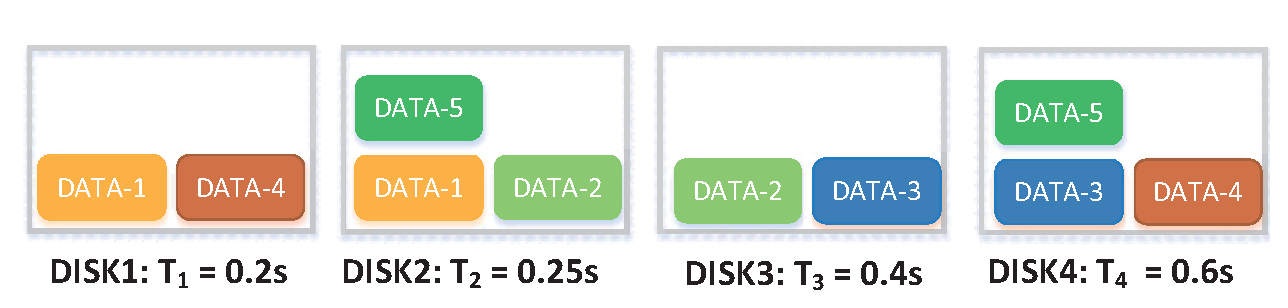
\includegraphics[height=0.8in]{fig1_10.eps}
	\caption{Distribution of five pieces of data across 4 disks.  }
	\label{fig1}
	\vspace{-0.4cm}
\end{figure}
\begin{figure}[!t]
	\centering
	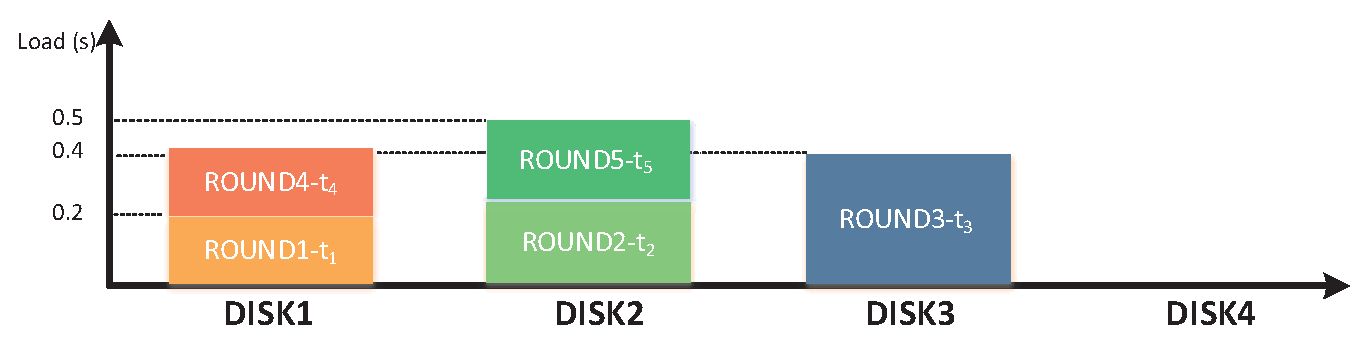
\includegraphics[height=0.8in]{fig2_4.eps}
	\caption{The process of WASH-greedy for the data distributed in Fig.~\ref{fig1}. }
	\label{fig2}
	\vspace{-0.4cm}
\end{figure}

Then, four tasks read data according to the strategy of \{$\left \langle 1, 1\right \rangle$, $\left \langle 2, 2\right \rangle$,  $\left \langle 3, 3\right \rangle$, $\left \langle 4, 1\right \rangle$, $\left \langle 5, 2\right \rangle$\}.The specific steps of WASH-greedy algorithm is shown in Fig.~\ref{fig2}.

Due to the fact that WASH-greedy always shows its preference on the disks with higher I/O performance for each task, such algorithm may easily overload high performance disks. Thus, WASH-greedy fails to  avoid the disks bottleneck, elongating the overall latency for data analytics.

\subsection{Randomized task scheduling}\label{Randomized}

%In the previous subsection \ref{Heuristic}, we explore a greedy heuristic algorithm to solve WASH problem, intuitively. 
%However, WASH-greedy could not avoid of the disk bottleneck while a lots of tasks are reading data from a high-performance disk. It is because that WASH-greed always giving preference to disks with high-performance as input for each task. Actually, such scenario are avoided if tasks could be allocated across disks, reasonably. 

In this subsection, we design a randomized algorithm, named $r$WASH, which avoids disk bottleneck by choosing source devices based on delicate calculated probabilities. Specifically, by relaxing the WASH problem to its relaxation version, i.e., WASH-relaxation, we use linear programming technique to solve WASH-relaxation. The solution obtained by linear programming technique, in a sense, represents the preference when selecting source disks. Therefore, our $r$WASH  uses such results as a series of probabilities to choose disk for each task. Subsequently, we prove that $r$WASH is concentrated on its optimum with high probability, i.e., 1- O($e^{-t^2}$), through our theoretical analysis, where $t$ is the concentration bound.



\paragraph{\textbf{Relaxation of WASH}} A linear programming (LP) problem is solvable within polynomial time as well as shows a lower bound for the corresponding integer linear programming (ILP) problem. A natural point of view is to relax the WASH problem to a LP problem. The method is to change the domain of decision variables from integer domain \{0, 1\} to real one [0, 1], i.e., WASH-relaxation. Such process is named $Relaxation$. Detailed description is illustrated as follows: 
%According to the previous analysis \ref{WASH}, this problem is NP-hard, whose optimal source disk for each task cannot be obtained within polynomial time. But 
%The solution of WASH-relaxation provides a lower bound for the original WASH problem (WASH is a minimization problem. For the maximization problem is on the contrary).
\vspace{-0.2cm}
 \begin{align}
 Min:&\;\;\;\;\;\max\limits_{i}\{\sum_{j}p_i^j*T_i\}\;\;\;\;\;\;[\rm{WASH-relaxation}]\nonumber\\
 s.t. 
 &\;\;\;\;\;\sum_{i}p_i^j = 1,\;\;\forall j,\nonumber\\
 &\;\;\;\;\;p_i^j \leq \pi_{\phi_j}^{i},\;\;\forall i,j,\nonumber\\
 &\;\;\;\;\;p_i^j \in[0, 1],\;\;\forall i,j.\nonumber
 \end{align}

Then, we use linear programming technique to solve WASH-relaxation whose solutions are fractions distributed in [0, 1]. In a sense, the fraction solutions represent the preference when choosing the source disk for each task. 

 \begin{algorithm}[!t]
 	%\renewcommand{\thealgorithm}{}
 	\textbf{Require:} Task-$j$ and its input data-$\phi_j$, $\forall j$. %and $d_i$ stores data $\phi_j$.
 	\begin{algorithmic}[1]	
 		\State $Result$ $\gets$ \{\}
 		\State \{$p_i^j$\} = WASH-relaxation		
 		
 		\leftline{\;\;\;\;\;\;$//$ \{$p_i^j$\} is the solution of WASH-relaxation problem. }
 		
 		\State Use \{$p_i^j$\} twice and get $<\{I_i^j\}_1, \{I_i^j\}_2 >$
 		
		\leftline{\;\;\;\;\;\;$//$ Apply rounding strategy twice. }
		\State Select $\{I_i^j\}$ from $<\{I_i^j\}_1, \{I_i^j\}_2>$

		\leftline{\;\;\;\;\;\;$//$ Select $\{I_i^j\}$ which minimizes WASH. }

 		\For{$\forall$ $i$, $j$, ($i \in \mathcal{D}$, $j \in \mathcal{T}$) } 
 			\If{$I_i^j$ == 1}
 			\State $Result$ $\gets$ $Result$ $\cup$ 	
 			\{$\left \langle j, i\right \rangle$\}
 			\EndIf
 		\EndFor	
 		\State Each task-$j$ reads data according to $Result$.
 	\end{algorithmic}
 	\caption{$r$WASH}\label{WASH-rdm}
 \end{algorithm}
 \paragraph{\textbf{$r$WASH schema}} 

Thus, our $r$WASH uses these fractions as probabilities to choose source disk for each task. In this way, the solution in fractional domain is mapped back to integer domain, which is named $Rounding$. 
Based on $Relaxation-Rounding$ strategy, we propose $r$WASH. 

The detailed of $r$WASH is shown in Algorithm \ref{WASH-rdm}. Line 1 initializes the set of $Result$. In line 2, we use linear programming technique to solve WASH-relaxation. For the third line, our proposed $r$WASH uses rounding strategy to convert fractional solutions into integer solutions. The specific rounding strategy is shown as follows:
 
The value of \{$p_i^j$\}  shows the correlation between task-$j$ and disk-$i$. Then, we select a disk-$i$ for each task-$j$ with the probability $p_i^j$. The method is that, $\forall j$, we randomly select a fraction $q_j$ from (0,1]. If $q_j$ $\in$ ($\sum\nolimits_{r = 1}^{k-1} p_{r}^{j}$,  $\sum\nolimits_{r = 1}^{k} p_{r}^{j}$], $2 \leq k \leq \mathcal{D} $, then $I_k^j = 1$, otherwise, $I_k^j$ = 0. This approach ensures only one disk can be selected for each task and $Pr[I_i^j = 1] = p_i^j$.
%Specially, if $q_j \leq p_{1}^{j}$, then $I_1^j = 1$ and $I_k^j$ = 0 ($k \in \mathcal{D} - \{ 1\}$).  For each task $t_j$, the corresponding decision variables are \{$p_0^j$,$p_i^j$, ..., $p_i^j$\}. 

In order to obtain more precise solution, we use rounding strategy twice, i.e., line 3. Then, we choose the one which minimizes the WASH between the two choices, i.e., power of two choices \cite{b43}. In lines 5-9, the results are stored in $Result$. After that, the tasks read the data according to $Result$. 

\begin{figure*}[!t]
	\centering
	\subfigure[Small Workload ]{\label{Fig:instance1}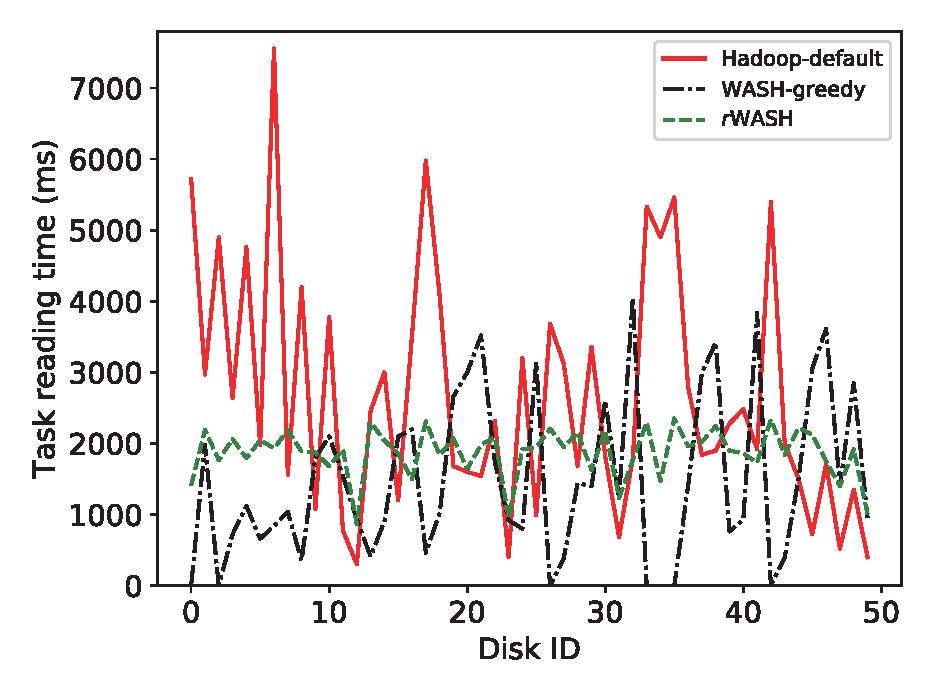
\includegraphics[height=1.55in]{fig_instance1_12.eps}}\quad\quad %quad 表示图像的间距
	\subfigure[Medium Workload ]{\label{Fig:instance2}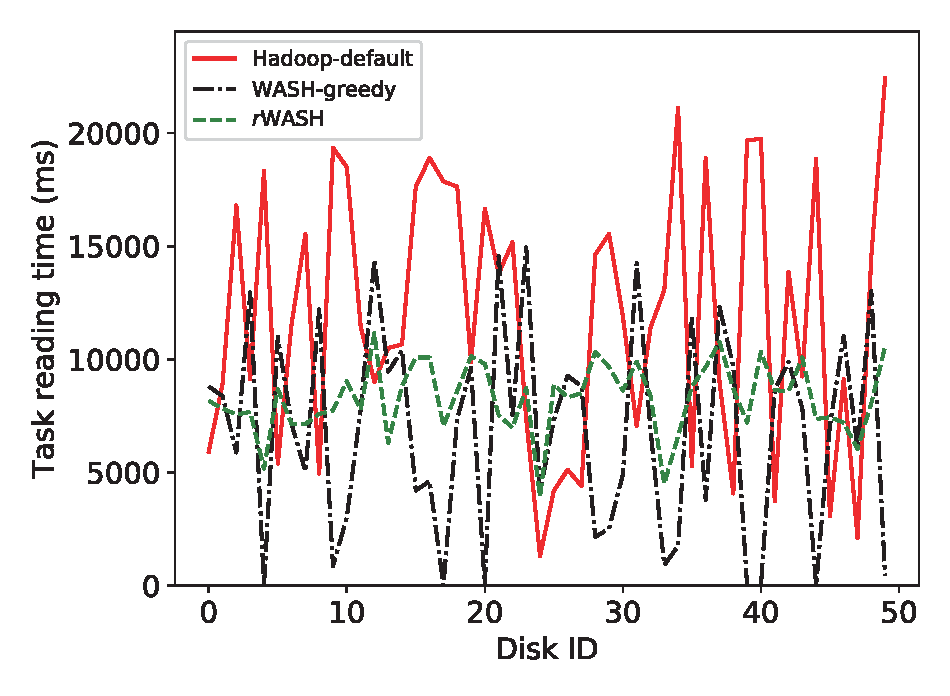
\includegraphics[height=1.55in]{fig_instance2_12.eps}}\quad\quad
	\subfigure[Large Workload
	]{\label{Fig:instance3}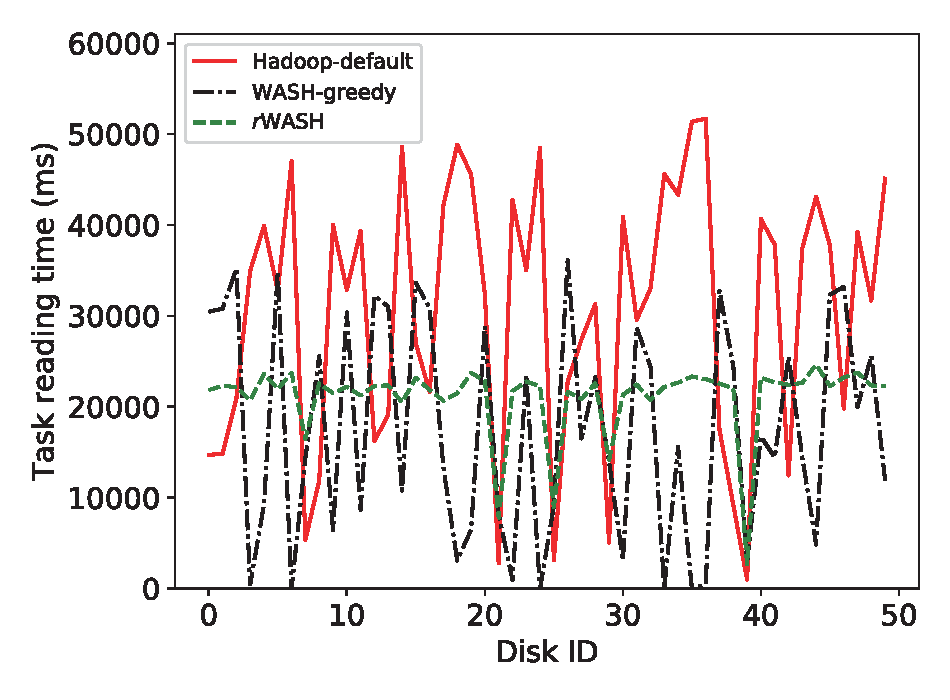
\includegraphics[height=1.5in]{fig_instance3_12.eps}}
	\vspace{-1ex}
	\caption{Characteristics of I/O workloads among 50 disks under different workloads. $r$WASH improves by up to 69\%, 50\% and 56\% over Hadoop-default, as well as 42\%, 25\% and 30\% over WASH-greedy in terms of the maximal task reading time for concurrent data fetching.}
	\label{Fig:instance}
%	\vspace{-1ex}
\end{figure*}
%\ref{Fig:instance1}, \ref{Fig:instance2} represents the results on Small Workload whose task number is 500. \ref{Fig:instance2} represents the results on Medium Workload whose task number is 2000. \ref{Fig:instance3} represents the results on Large Workload whose task number is 5000. X-axis represents the disk ID. Y-axis represents the load of each disk, i.e., the total tasks reading time on each disk.
\section{Analysis of Algorithm $r$WASH}\label{Analysis}

In this section, we will show that our $r$WASH is concentrated on its optimum with high probability, i.e., 1- O($e^{-t^2}$), through our theoretical analysis, where $t$ is the concentration bound. Firstly, we prove that the difference between disk-$i$'s reading time contributed by any task-$j$ and its expectation could be bounded through Martingale Analysis \cite{b12}. After that, we use Azuma's Inequality to illustrate the gap between the feasible solution and the optimal solution. For simplification, we use $SOL$ to represent the feasible solution solved by $r$WASH, and $OPT$ to represent the optimal solution of WASH problem in the following.

\vspace{0.2cm}
\emph{\textbf{Theorem 2:}} $Pr[SOL - OPT\leq t] \geq 1 - O(e^{-2t^2})$.

\emph{\textbf{Proof:}} Firstly, the contribution on additional workload of each task-$j$ to disk-$i$'s $load$ is expressed as
\vspace{-0.1cm}
 \begin{align}
&\;\;\;\;\;Z_i^j = I_i^j*T_i.
\end{align}

\vspace{-0.2cm}
From the rounding strategy in Algorithm \ref{WASH-rdm}, we obtain
 \vspace{-0.2cm}
 \begin{align}
&\;\;\;\;\;Pr[I_i^j = 1] = p_i^j. \nonumber
\end{align}
%Therefore

\vspace{-0.2cm}
The expectation of $Z_i^j$ then is represented as
\vspace{-0.2cm}
\begin{align}
E[Z_i^j] &= E[I_i^j]*T_i \nonumber\\
&= (Pr[I_i^j = 1] * 1 +  0)*T_i = p_i^j*T_i.\label{prove:expect}
\end{align}

\vspace{-0.2cm}
The difference between disk-$i$'s reading time contributed by any task-$j$, i.e., $Z_i^j$, and its expectation, i.e., $E[Z_i^j]$, is defined as
 \vspace{-0.1cm}
\begin{align}
Q_i^j = Z_i^j - E[Z_i^j].\label{prove:diff}
\end{align}

%we denote by $L_i^{\mathcal{|T|}}$ the sum of $Q_i^j$ in disk $i$, i.e., 
\vspace{-0.2cm}
%For each disk-$i$, we denote by $L_i^{\mathcal{|T|}}$ the sum of the difference between $Z_i^j$ and $E[Z_i^j]$, i.e., $Q_i^j$, 
For each disk-$i$, we denote by $L_i^{\mathcal{|T|}}$ the sum of $Q_i^j$, $\forall j \in \mathcal{T}$, i.e., 
 \vspace{-0.1cm}
\begin{align}
L_i^{\mathcal{|T|}} = \sum\nolimits_{j = 1}^{\mathcal{|T|}} Q_i^j
=  L_i^{\mathcal{|T|} - 1} + Q_i^{\mathcal{|T|}}. \label{prove:L_margin}
\end{align}

Then, the expectation of $L_i^{r}$, on the condition $L_i^{1}$, $L_i^{2}$, ..., $L_i^{r-1}$ ($r \geq 1$), is represented as follows:
\vspace{-0.1cm}
\begin{align}
&E[L_i^{r}|L_i^{1}, L_i^{2}, ..., L_i^{r-1}] \nonumber\\
&\overset{\text{(8a)}}{=}E[L_i^{r-1} + Q_i^{r} |L_i^{1}, L_i^{2}, ..., L_i^{r-1}] \nonumber\\
&\overset{\text{}}{=}E[L_i^{r-1} |L_i^{1}, L_i^{2}, ..., L_i^{r-1}]
+ E[Q_i^{r} |L_i^{1}, L_i^{2}, ..., L_i^{r-1}] \nonumber\\
&\overset{\text{(8b)}}{=}L_i^{r-1} + E[Z_i^r - E[Z_i^r] |L_i^{1}, L_i^{2}, ..., L_i^{r-1}]\nonumber\\
&=L_i^{r-1} + E[Z_i^r|L_i^{1}, L_i^{2}, ..., L_i^{r-1}]
-E[E[Z_i^r] |L_i^{1}, L_i^{2}, ..., L_i^{r-1}]\nonumber\\
&=L_i^{r-1} + E[Z_i^r] - E[Z_i^r]\nonumber\\
&=L_i^{r-1}.\label{prove:marginsq}
\end{align}

\vspace{-0.2cm}
The Equation (8a) and Equation (8b) hold due to Equation (\ref{prove:L_margin}) and Equation (\ref{prove:diff}), respectively. Due to the fact that $E[L_i^{r}|L_i^{1}, L_i^{2}, ..., L_i^{r-1}] = L_i^{r-1}$, we conclude that $L_i^{1}$, $L_i^{2}$, ..., $L_i^{|\mathcal{T}|}$ is a martingale sequence \cite{b13}. For completeness, we let $L_i^{0}$ = 0. After considering each item and the relationship between two consecutive items in such martingale sequence, $\forall r \geq 1$, we have
\vspace{-0.2cm}
\begin{align}
  |L_i^r - L_i^{r-1}|&\overset{\text{(9a)}}{=} |Q_i^{r}| \overset{\text{(9b)}}{=} |Z_i^r - E[Z_i^r]|\leq g_i^r, \label{prove:bound1}\\
  g_i^r &= \max\{T_i -  E[Z_i^r], E[Z_i^r]\}.\label{prove:bound}
\end{align}

\vspace{-0.15cm}
Equation (9a) and (9b) hold due to Equation (\ref{prove:L_margin}) and Equation (\ref{prove:diff}), respectively. For given $p_i^j$, $T_i$ and $E[Z_i^r]$ are both constant. Thus, in Equation (\ref{prove:bound}), the difference of any two consecutive items, i.e., $L_i^r$ and $L_i^{r-1}$, $\forall r \geq 0$, in the martingale sequence, has a constant bound, i.e., $g_i^r$. Based on Equation (\ref{prove:marginsq}), Equation (\ref{prove:bound}) and Azuma's Inequality, we have
\vspace{-0.3cm}
\begin{align}
Pr\{L_i^{|\mathcal{T}|} - L_i^{0} \geq t\} \leq exp\{-\frac{t^2}{2\sum_{ i = 1 }^{|\mathcal{T}|}(g_i^k)^2}\}. \label{prove:azuma}
\end{align}

\vspace{-0.1cm}
Substituting Equation (\ref{prove:diff}) and Equation (\ref{prove:L_margin}) into the  Equation (\ref{prove:azuma}), we have  
\vspace{-0.2cm}
\begin{align}
Pr\{\sum\nolimits_{j = 1}^{|\mathcal{T}|} Z_i^j - 
	\sum\nolimits_{j = 1}^{|\mathcal{T}|} E[Z_i^j]\geq t\} \leq exp\{-\frac{t^2}{2\sum_{ i = 1 }^{|\mathcal{T}|}(g_i^k)^2}\},\nonumber
\end{align}
 \vspace{-0.2cm}
 where it equals to
\begin{align}
Pr\{\sum_{j = 1}^{|\mathcal{T}|} Z_i^j \leq \sum_{j = 1}^{|\mathcal{T}|} E[Z_i^j] + t\} & \geq 1 - exp\{-\frac{t^2}{2\sum_{ i = 1 }^{|\mathcal{T}|}(g_i^k)^2}\}\nonumber\\
& = 1 - O(e^{-t^2}).\label{prove:azuma3}
\end{align}

\vspace{-0.2cm}
For simplification, we take $S_i$  = $\sum_{j = 1}^{|\mathcal{T}|} Z_i^j$,
$E_i$ = $\sum_{j = 1}^{|\mathcal{T}|} E[Z_i^j]$
$\overset{\text{(12a)}}{=}$
$\sum_{j = 1}^{|\mathcal{T}|} p_i^j*T_i$, where (12a) holds due to Equation (\ref{prove:expect}). After substituting $S_i$ and $E_i$ into Inequality (\ref{prove:azuma3}), we have
\vspace{-0.2cm}
\begin{align}
Pr\{S_i \leq E_i + t\} \geq 1- O(e^{-t^2}). \label{prove:SU}
\end{align}

\vspace{-0.2cm}
$S_i$ represents the actual load of disk-$i$, and $E_i$ denotes the solution of LP as well as the expectation load of disk-$i$. Since LP provides a lower bound of the ILP problem (WASH is a minimization problem), $\forall x \in \mathcal{D}$, we have
\vspace{-0.2cm}
\begin{align}
E_x \leq OPT.\label{prove:OPT}
\end{align}

\vspace{-0.2cm}
Without losing generality, $u$ and $v$ represent the indexes of the maximal $S_i$ and $E_i$, respectively, i.e.,
\vspace{-0.2cm}
\begin{align}
	S_u = S_{max} = \max\nolimits_i S_i,\\
	E_v = E_{max} = \max\nolimits_i E_i.\label{prove:Emax}
\end{align}

\vspace{-0.2cm}
Then, we have the following inequalities,
\vspace{-0.2cm}
\begin{align}
SOL = S_u  
\overset{\text{(18a)}}{\leq} E_u+t
\overset{\text{(18b)}}{\leq} E_v+t
\overset{\text{(18c)}}{\leq} OPT+t.\label{prove:SOL-OPT}
\end{align}
%OPT(\text{WASH}) QoS-aware Data Replica Recovery Algorithm in Cloud System

Inequality (18a), (18b) and (18c) hold due to Inequality (\ref{prove:azuma3}), Equation (\ref{prove:Emax}) and Inequality (\ref{prove:OPT}), respectively.  Based on Inequality (\ref{prove:SU}) and Inequality (\ref{prove:SOL-OPT}), we conclude that
\vspace{-0.1cm}
\begin{align}
Pr\{SOL<OPT+t\}\geq 1 - O(e^{-t^2}).\label{prove:result}
\end{align}

\vspace{-0.2cm}

Then, the result of Inequality (\ref{prove:result}) can be improved to $1 - O(e^{-2t^2})$ by applying power of two choices, i.e., in lines 3-4 of $r$WASH. In practice, for given probability, e.g., $1 - O(e^{-2t^2}) = 0.85$, when hundreds of tasks are deployed, $t$ is acceptable. \hfill \;$\qedsymbol$
%More   served from the equation (\ref{prove:result}), the feasible solution, i.e., $SOL$ found by the $r$WASH and the optimum, i.e., $OPT$  are approximated by probability $1 - O(e^{-t^2})$.
%, i.e., only a few millisecond.

\section{PERFORMANCE EVALUATION}\label{PERFORMANCE_EVALUATION}
%, with $r$WASH and storage-unaware scheduling algorithm.
In this section, we conduct extensive simulations for evaluating $r$WASH. The results of our extensive simulations show that $r$WASH improves by up to 55\% and 30\%, respectively, compared with typically and widely used storage-unaware scheduling algorithm as well as WASH-greedy.

\subsection{Simulation Setup}\label{SCM}
Traditional scheduling mechanisms are often unaware of the types and I/O workloads of storage devices. For example, the default scheduler in Hadoop, whose abbreviation is Hadoop-default, selects source devices storing the related data of tasks randomly. In our extensive simulations, we compare $r$WASH with WASH-greedy and Hadoop-default for evaluation.

\textbf{Workloads:} According to the characteristics of Google traces \cite{b20}, we classify the workloads into three categories: Small, Medium and Large. In small workload, most of the jobs have 1-150 tasks. In Large Workload, there are 50\% of the jobs that own at least 500 tasks. And, the Medium Workload is in the middle of them in terms of the task number.
%as shown in TABLE \ref{tab:workload}


\begin{figure*}[!t]
	\centering
	\subfigure[Results under various I/O workloads ]{\label{Fig:completeWorkload}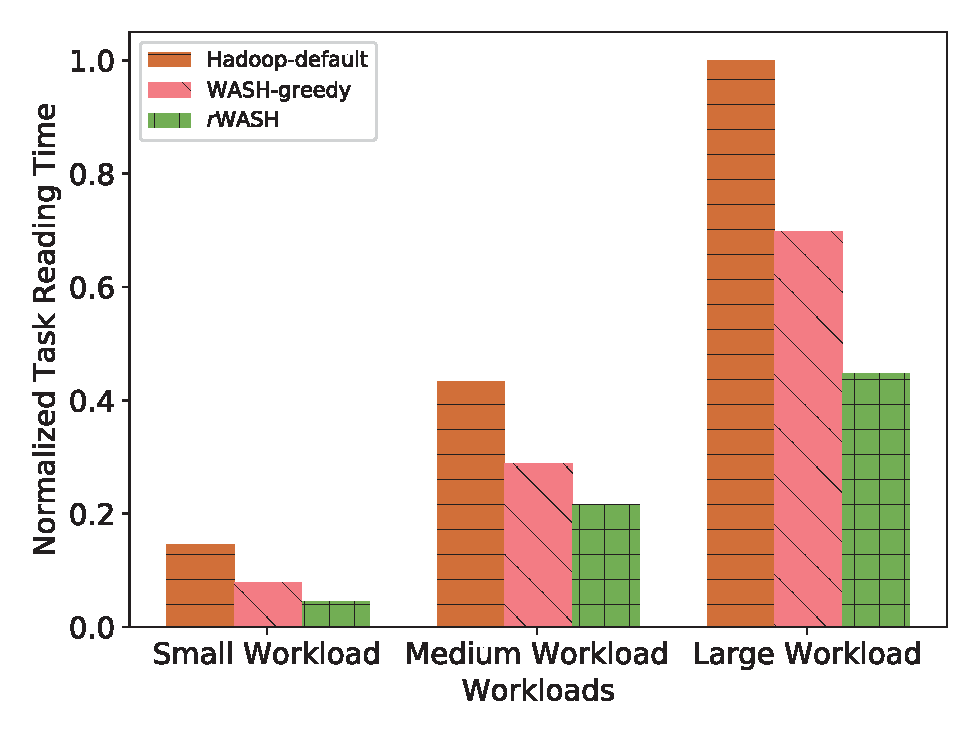
\includegraphics[height=1.6in]{figcomplete1_8.eps}}\quad\quad %quad 表示图像的间距
	\subfigure[Results under various I/O performance]{\label{Fig:completeHeter}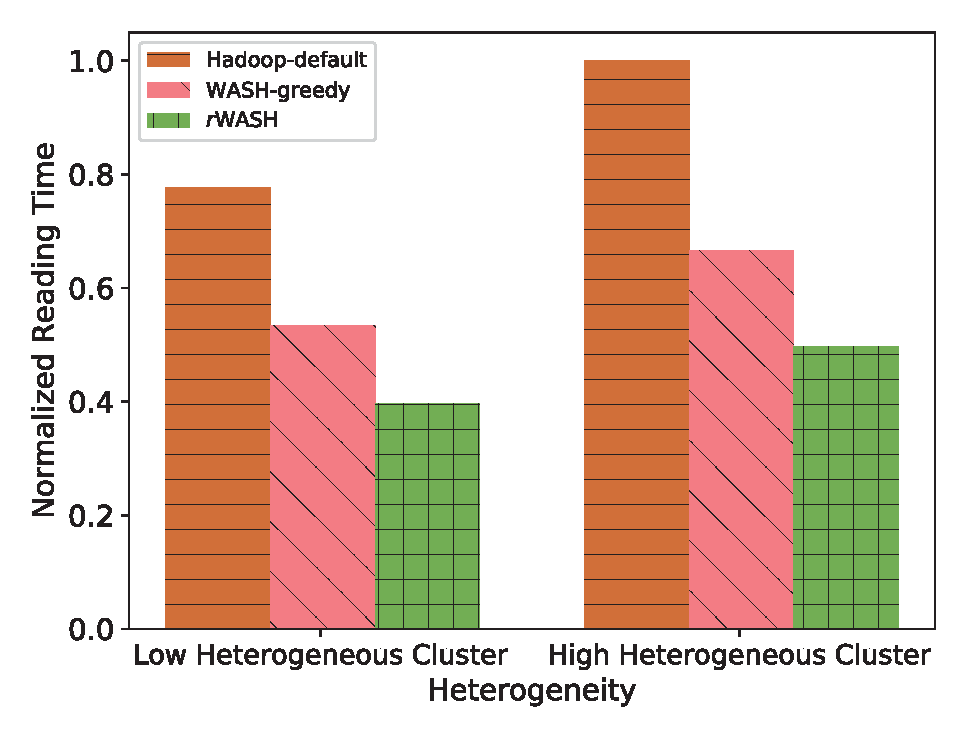
\includegraphics[height=1.6in]{figcomplete2_8.eps}}\quad\quad
	\subfigure[Results under various number of data replica
	]{\label{Fig:completeRep}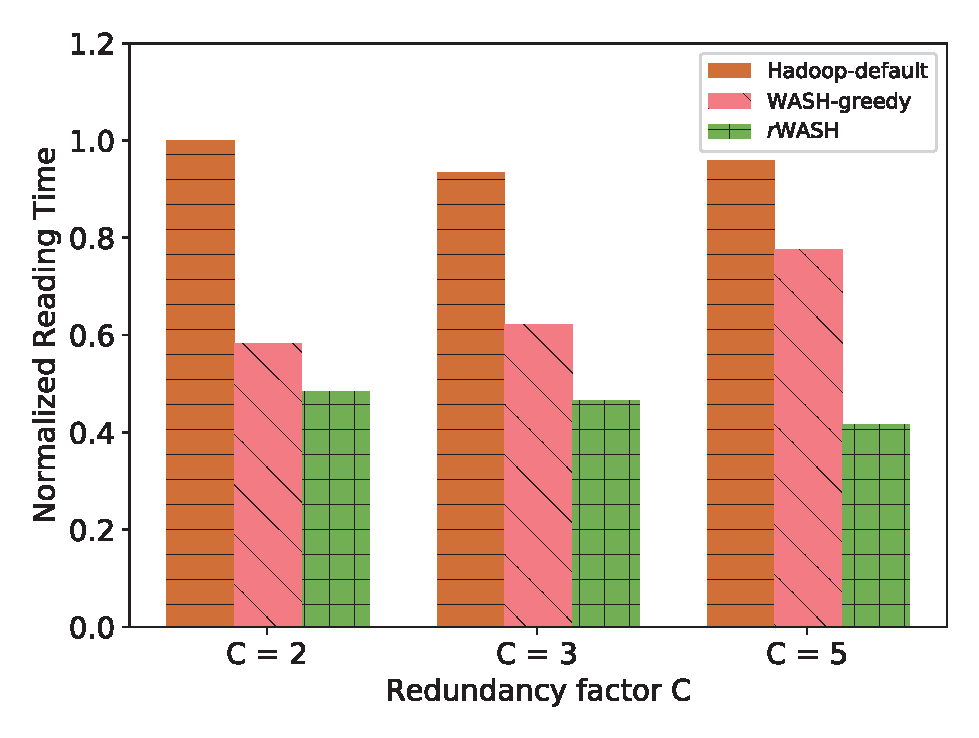
\includegraphics[height=1.6in]{figcomplete3_8.eps}}
	\vspace{-1ex}
	\caption{Results under various scenarios with different I/O workloads, I/O performance and the number of data replicas. $r$WASH improves 58\%, 50\% and 53\% over Hadoop-default, as well as 34\%, 26\% and 30\% over WASH-greedy in terms of the maximal task reading time.}
	\label{Fig:complete}
	%\vspace{-1ex}
\end{figure*}
% \ref{Fig:completeWorkload} represents effect of different workloads on reading time. \ref{Fig:completeHeter} represents the reading time of the three algorithm on different Heterogeneity cluster. \ref{Fig:completeRep} denotes the reading time of the three algorithm when $C$ is different.

%\ref{Fig:completeWorkload} represents effect of different workloads on reading time. \ref{Fig:completeHeter} represents the reading time of the three algorithm on different Heterogeneity cluster. \ref{Fig:completeRep} denotes the reading time of the three algorithm when $C$ is different. Y-axis denotes the reading time of all tasks which has been normalized.

\begin{figure*}[!t]
	\centering
	\subfigure[Small Workload ]{\label{Fig:unbalance1}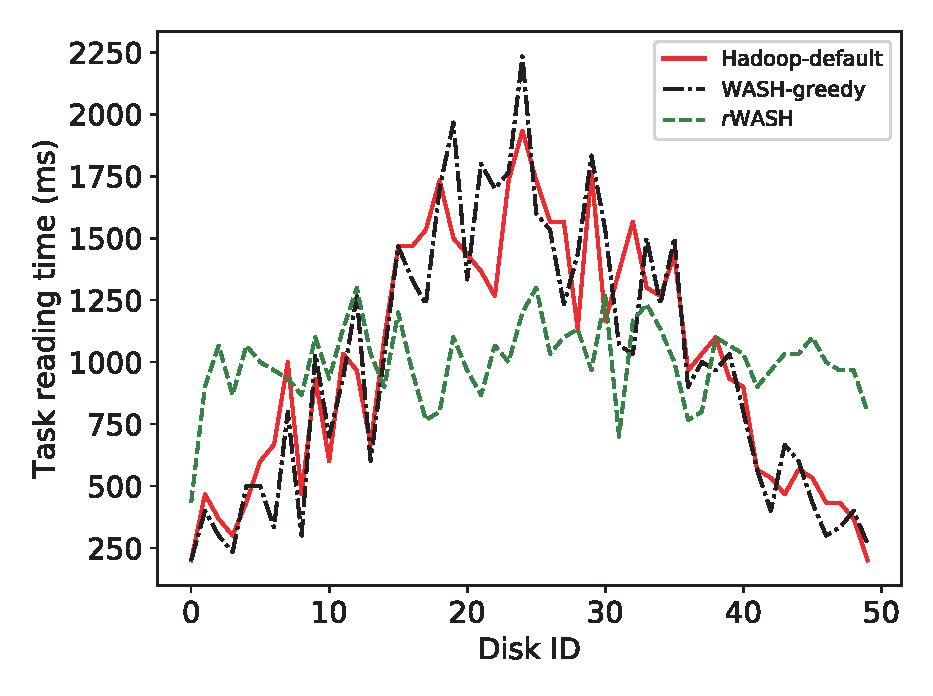
\includegraphics[height=1.6in]{fig_unbanlancedata1_1.eps}}\quad\quad %quad 表示图像的间距
	\subfigure[Medium Workload ]{\label{Fig:unbalance2}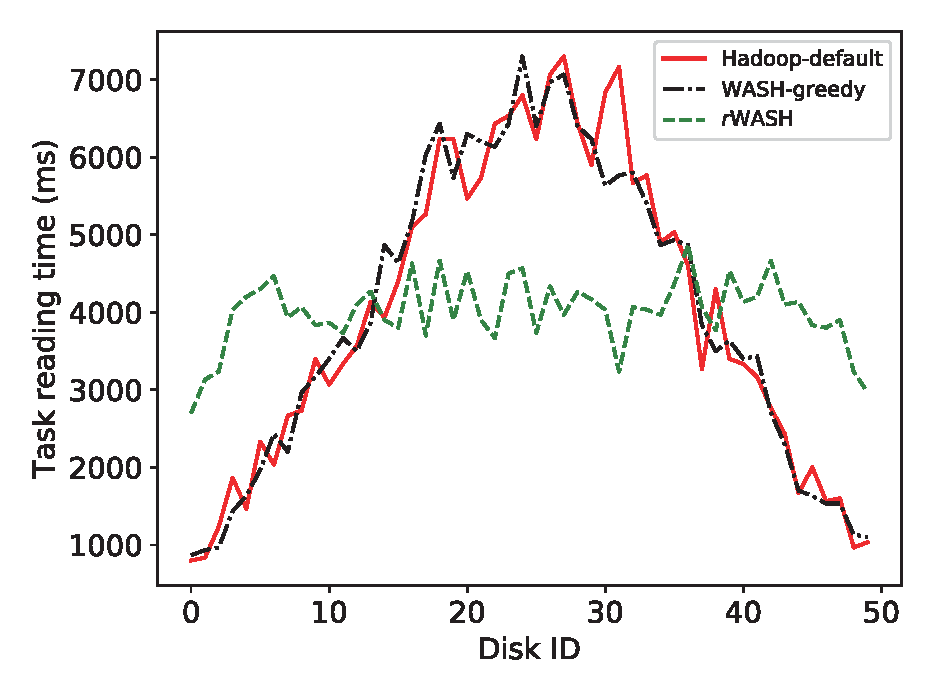
\includegraphics[height=1.6in]{fig_unbanlancedata2_1.eps}}\quad\quad
	\subfigure[Large Workload
	]{\label{Fig:unbalance3}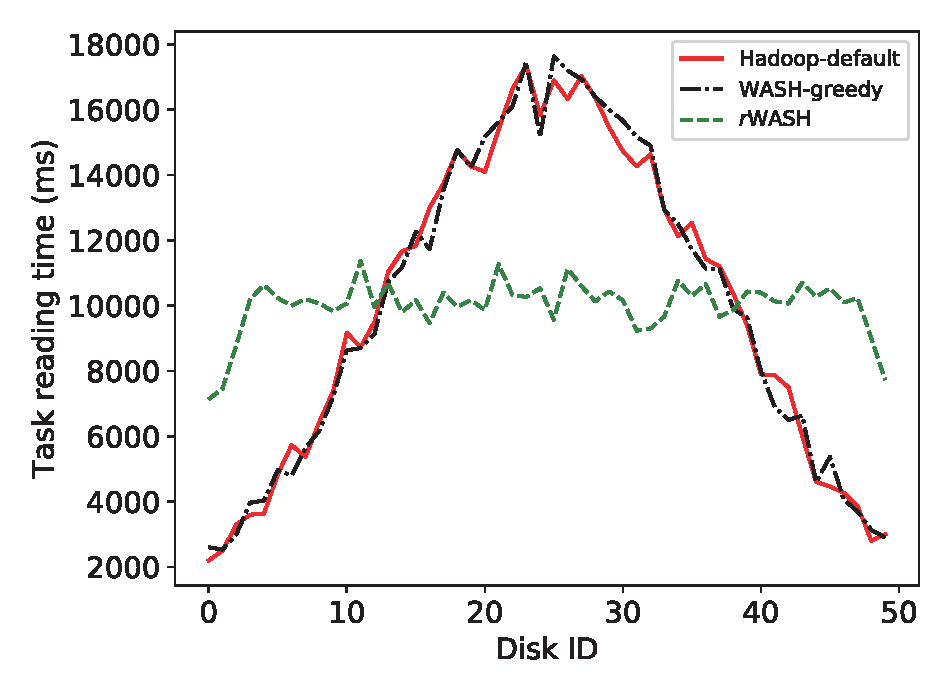
\includegraphics[height=1.6in]{fig_unbanlancedata3_1.eps}}
	\vspace{-1ex}
	\caption{Results for various I/O workloads under skewed data distribution. Our $r$WASH improves by up to 27\%, 41\% and 34\% over Hadoop-default, as well as 38\%, 32\% and 37\% over WASH-greedy in terms of the maximal task reading time.
	}
	\label{Fig:unbalance}
	\vspace{-0.35cm}
\end{figure*}

%\ref{Fig:instance1} represents the results on Small Workload whose task number is 500. \ref{Fig:instance2} represents the results on Medium Workload whose task number is 2000.\ref{Fig:instance3} represents the results on Large Workload whose task number is 5000.  X-axis represents the disk ID. Y-axis represents the load of each disk, i.e., the total tasks reading time on each disk.

%\begin{table}[htbp]
%	\caption{THE DIFFERENT TRACES USED FOR EXPERIMENT}
%	\begin{center}
%		\begin{tabular}{|c|c|c|c|}
%			\hline
%			 \diagbox{Traces}{Number of tasks} & 1-150 & 150-500 & $\ge$ 500\\
%			\hline
%			Small Workload & 96\% & 2\% & 2\%\\
%			\hline
%			Medium Workload & 50\% & 40\% & 10\%\\
%			\hline
%			Large Workload & 40\% & 10\% & 50\%\\
%			\hline
%		\end{tabular}
%		\label{tab:workload}
%		\vspace{-0.4cm}
%	\end{center}
%\end{table}

\textbf{Settings:}
In traditional distributed file systems, e.g., HDFS\cite{b19}, distributed datasets, i.e., data blocks, are uniformly stored among disks, whose unified size is 128MB. Therefore, in this experimental environment, we uniformly deploy 200000 data blocks among 500 disks, each of which has three data replicas. The task reading time for only one piece of data, i.e., $T_i$, ranges from 100ms to 500ms, uniformly. 



\subsection{Simulation Results}

\textbf{Characteristics of I/O workloads:} Fig.~\ref{Fig:instance} shows the results under various workloads among 50 disks. X-axis represents the IDs for different disks while Y-axis represents the task reading time. Note that the completion of concurrent data fetching relies on the maximal task reading time. The black dotted line illustrates the result of WASH-greedy while the green line illustrates the result of $r$WASH. In general, $r$WASH performs much better than Hadoop-default in terms of the maximal task reading time. As shown in Fig.~\ref{Fig:instance1} further, i.e., in the small workload scenario, the result of Hadoop-default has large fluctuations since it is unaware of storage types and unbalance I/O workloads among heterogeneous storage devices when selecting a source device for each task. As a result, the straggler elongates the completion time for concurrent data fetching, although the data is distributed uniformly among storage devices.

More specifically, the maximal task reading time under Hadoop-default is 7560ms since the bottleneck occurs within disk-6 for concurrent data fetching, and further influences the overall latency of data analytics, as shown in Fig.~\ref{Fig:instance1}. Although WASH-greedy reduces the maximal task reading time to 4050ms, it ignores to avoid the hotspots on those disks with higher I/O performance. WASH-greedy actually shows its preference on the disk with higher I/O performance for data fetching, but crowded I/O workloads also worsen the task reading time due to the concurrent use. In contrast, $r$WASH selects the source devices based on delicate calculated probabilities with peak 2340ms in disk-17. 
Compared with Hadoop-default and WASH-greedy, $r$WASH reduces reading time for tasks by up 69\% and 42\%, respectively.   

Further shown in Fig.~\ref{Fig:instance2} and Fig.~\ref{Fig:instance3}, with the increase number of concurrent data fetching, the maximal task reading time also increases among disks. When the number of tasks is about 2000 in middle workload scenario, the maximal task reading time of 
Hadoop-default and WASH-greedy is 22440ms and 14950ms, respectively. The maximal task reading time of $r$WASH is only 11160ms, which speeds up the concurrent data fetching by up to 50\% and 25\%, respectively. 
Furthermore, in large Workloads scenario, $r$WASH reduces reading time for tasks by up to 56\% and 30\% over Hadoop-default and WASH-greedy, respectively. 

 %5546, 3650 and 2346

\textbf{Scalability of $r$WASH:} Next, we evaluate $r$WASH from three main aspects, including I/O workloads, I/O performance and the number of data replicas. In Fig.~\ref{Fig:completeWorkload}, it summarizes the maximal task reading time for three I/O workloads, illustrating that the average improvement of $r$WASH compared with other two strategies is at least 34\%. In Fig.~\ref{Fig:completeHeter}, when the average I/O performance is high, i.e., the average reading time for one data block from disks is only 150ms in the scenario of low heterogeneity, the reduction of task reading time by $r$WASH compared with Hadoop-default and WASH-greedy is 49\% and 26\%, respectively. When the average I/O performance is low, i.e., the average reading time for only one data block from disks is 300ms in the scenario of high heterogeneity, the reduction by $r$WASH compared with Hadoop-default and WASH-greedy is 51\% and 25\%, respectively.

As shown in Fig.~\ref{Fig:completeRep}, with the growth on the number of data replicas, the maximal task reading time for Hadoop-default and $r$WASH decreases while the maximal task reading time for WASH-greedy increases instead. The reason behind is that for large number of data replicas, more data is likely to be stored within those disks with high I/O performance. Thus, WASH-greedy leaves much heavier I/O workloads on those disks since it often shows its preference on those disks, making them being hotspots and elongating the maximal task reading time due to the concurrent use. Fortunately, for $r$WASH, it has more choices among heterogeneous disks and has more opportunities to balance the I/O workloads for data analytical tasks. In general, $r$WASH takes not only the I/O performance of disks but also the I/O workloads into consideration, and is willing to choose almost the best source disk for each task. $r$WASH improves up to 57\% deduction on task reading time when the number of data replicas is 5.

 \textbf{Impact of data distribution:} Fig.~\ref{Fig:unbalance} shows the results for various I/O workloads under skewed data distribution. More technically, the data is unbalanced stored among disks, which might obey Gaussian distribution \cite{b44}. The skewed data distribution actually influences the maximal task reading time because more data is crowded within a few disks. For Hadoop-default and WASH-greedy, the feasible choices of source disks become small, and hence more I/O workloads are crowded within these disks with high I/O performance, incurring high task reading time. For $r$WASH, it is willing to choose those with poor I/O performance for offloading. In general, $r$WASH improves by up to 27\%, 41\% and 34\% over Hadoop-default, as well as 38\%, 32\% and 37\% over WASH-greedy, respectively.


In general, $r$WASH takes only several seconds for computation, i.e., the linear programming part in $r$WASH, which is acceptable for realistic deployment. The overall average improvement compared with $r$WASH and Hadoop-default as well as WASH-greedy is 55\% and 30\%, respectively.


\section{CONCLUSION}\label{CONCLUSION}
In this paper, in order to avoid the unbalanced use on fetching large volume of data concurrently from heterogeneous storage devices as well as to speed up the task reading time for data analytics, the types of these storage devices and the I/O workloads should be both taken into consideration. Therefore, we formulate the Workload-Aware Scheduling problem for Heterogeneous storage devices (WASH), and design a randomized algorithm ($r$WASH). $r$WASH chooses source device for each task based on delicate calculated probabilities and can be proved concentrated on its optimum with high probability through our theoretical analysis. The results of our extensive simulations show that $r$WASH improves by up to 55\% over the art-of-the-state baseline algorithm.
%showing its NP-hardness
%\section*{Acknowledgment}
%None
\begin{comment} ... 
\section*{APPENDIX}

\textbf{\normalsize{The Proof of Theorem 1}}
\vspace{1ex}

The decision version of our WASH problem asks whether there exists a series of variables satisfying all the constrains (there is no objective function). Such problem can be reduced from 3-SAT problem which is defined as follows: Given a set of variables $B = \{b_1, b_2, ..., b_n\}$, each of them only can be taken in $\{True, False\}$. A literal $l$ consists of $b_i$ or $\overline b_i$. There are $m$ different clauses $C_j$, one of which is a disjunction of three literals \cite{b44}. The 3-SAT problem asks whether or not there exits a series of $b_i$ satisfying the total clauses which is one of Karp's 21 NP-complete problems \cite{b9}.

Taking the special case of  WASH problem, the parameters are set as follows:
\begin{itemize}
	\item $\mathcal{D}$ = \{1, 2, ..., 3\};
	$\mathcal{M}$ = \{1, 2, ..., n\}; 
	\item $C$ = 3.
\end{itemize}

Each variable $b_i$ has corresponding variable $I_l$.
For each clause like $b_1\wedge  b_2 \wedge b_3$, we have $I_1 + I_2 + I_3 = 1$. On one hand, if there exits a series of $b_i \in \{True, False\}$ satisfying the clauses, the constrains of WASH could be satisfied. On the other hand,  if there exits a series of $I_i \in \{1, 0\}$ satisfying the our constrains, the clauses of 3-SAT could be satisfied. \hfill \qedsymbol


The decision version of WASH problem is formulated as: Whether the optimum of WASH problem is less than $K$ or not.


The canonical form \cite{b11} of ILP is described below.

For $m\times n$ matrix \textbf{A}
\begin{align}
Min:&\;\;\;\;\;\textbf{c}^T\textbf{x}\;\;\;\;\;\;[\rm{ILP}]\label{ILP}\\
s.t. 
&\;\;\;\;\;\textbf{A}\textbf{x}\geq \textbf{b},\nonumber\\
&\;\;\;\;\;\textbf{x} \geq0\;and\;\textbf{x} \in \mathbb{Z}^n.\nonumber
\end{align}
Taking the special case of WASH problem, the parameters are set as follows:
\begin{itemize}
	\item $\mathcal{D}$ = \{$0$, $1$, $2$\};$T_0$ = 1, $T_1$ = 1, $T_2$=1; $\mathcal{M}$ = \{$0$, $1$, ..., $n-1$\}; $C$ = 3
	\item $T$ = \{$0$, $1$, ..., $n-1$\}
\end{itemize}

It means that there are 3 disks, $0$, $1$, $2$, in the data center, each disk with a $T_i$ of 1. A total of n data, and each data has three replicas which deployed in the three disks, respectively. When the query job arrives, the job is divided into n tasks, \{$t0$, $1$, ..., $n$\} to read n data, \{$0$, $1$, ..., $n$\}, respectively.

For this particular case, the problem description can be modified to:
\begin{align}
Min:&\;\;\;\;\;\max\{\sum_{j}I_0^j, \sum_{j}I_1^j, \sum_{j}I_2^j\}\;\;\;\;\;[\rm{WASH-sp}]\nonumber\\
s.t. 
&\;\;\;\;\;I_0^j + I_1^j +I_2^j= 1,\;\;\forall j,\nonumber\\
&\;\;\;\;\;I_0^j, I_1^j, I_2^j\in\{0,1\},\;\;\forall j \in[0,n).\nonumber
\end{align}

Let  $x$ = $\sum_{j}I_0^j$, $y$ = $\sum_{j}I_1^j$, $z$ = $\sum_{j}I_2^j$, and the problem description can be modified to:
\begin{align}
Min:&\;\;\;\;\;\max\{x,y,z\}\;\;\;\;\;\;[\rm{WASH-sp}]\\
s.t. 
&\;\;\;\;\;x + y + z = n,\;\label{enlarge-cons}\\
&\;\;\;\;\;0 \leq x, y, z \leq n  \;\;x, y, z\in\mathbb{Z}.\nonumber
%&\;\;\;\;\;0 \leq y \leq n, y\in\mathbb{Z}\nonumber\\
%&\;\;\;\;\;0 \leq z \leq n, z\in\mathbb{Z}\nonumber
\end{align}
In the minimization problem, x + y + z = n can be modified to x + y + z = n and let $R$ denotes $\max\{x,y,z\}$. 

Finally, WASH-sp problem is converted to:
\begin{align}
Min:&\;\;\;\;\;0*x+0*y+0*z+R\;\;\;\;\;\;\;[\rm{WASH-ILP}]\label{WASH-ILP}\nonumber\\
s.t. 
&\;\;\;\;\;x + y + z \geq n,\;\nonumber\\
&\;\;\;\;\;-x + R \geq 0, \nonumber\\
&\;\;\;\;\;-y + R \geq 0, \nonumber\\
&\;\;\;\;\;-z + R \geq 0, \nonumber\\
&\;\;\;\;\;0 \leq x, y, z \leq n  \;\;x, y, z\in\mathbb{Z},\nonumber\\
%&\;\;\;\;\;0 \leq x \leq n, x\in\mathbb{Z}\nonumber\\
%&\;\;\;\;\;0 \leq y \leq n, y\in\mathbb{Z}\nonumber\\
%&\;\;\;\;\;0 \leq z \leq n, z\in\mathbb{Z}\nonumber\\
&\;\;\;\;\;R \geq 0, R\in\mathbb{Z}.\nonumber
\end{align}
%(\ref{WASH-ILP})
Obviously, WASH-ILP  is an instance of ILP in (\ref{ILP}). The decision version of 0-1 ILP (A variation in which only the restrictions must be satisfied, without optimization) is one of Karp's 21 NP-complete problems \cite{b9}, so ILP is NP-hard. Further, the WASH-ILP problem is NP-hard.

On the one hand, when the optimal solution of WASH-ILP problem is obtained, the corresponding {x, y, z} can be converted into variable {$I_i^j$} thin polynomial time by setting the value in \{$I_0^0$, $I_0^1$, ...,$I_0^{x-1}$, $I_1^{x}$, $I_1^{x+1}$, ..., $I_1^{x+y-1}$, $I_2^{x+y}$, $I_1^{x+y+1}$, ..., $I_2^{x+y+z-1}$\} to be 1, which will make the corresponding WASH-sp problem obtain the optimal solution. On the other hand, when the variable \{$I_i^j$\} make the WASH-sp problem obtain the optimal solution, the WASH-ILP also obtains the optimal solution by setting $x$ = $\sum_{j}I_0^j$, $y$ = $\sum_{j}I_1^j$, $z$ = $\sum_{j}I_2^j$. It can be seen from the above that any solution can be polynomially transformed between the WASH-sp and WASH-ILP. Therefore, WASH-sp is NP-hard. 

As a result of that WASH-sp is a special case in WASH, WASH problem is NP-hard.\hfill $\qedsymbol$
\end{comment}

\begin{small}
	\bibliographystyle{IEEEtran}
	\bibliography{DLP}
\end{small}




\end{document}

